\section{Synthesis design (Route C): from factor chain to a TpPa-1 protocol}
\label{sec:routec}

This section converts the survey's evidence into a decision-recorded synthesis plan for the
$\beta$-ketoenamine COF TpPa-1 (monomers: 1,3,5-triformylphloroglucinol, Tp; and
\emph{p}-phenylenediamine, Pa-1; stoichiometry 2\,Tp\,:\,3\,Pa-1 from the 3$\times$CHO /
2$\times$NH$_2$ functional balance)~\cite{kandambeth2012construction}. The full
safety-annotated protocol, candidate-route decision table, and machine-readable experiment plan
are deliverable artifacts of this project;\footnote{Artifacts:
\texttt{ideas/route\_c\_synthesis\_plan.md} and \texttt{ideas/experiment\_route\_c\_tppa1.json}
in the project workspace.} this section presents the decision logic and the quantitative core. Figure~\ref{fig:route} shows the route.

\begin{figure}[t]
  \centering
  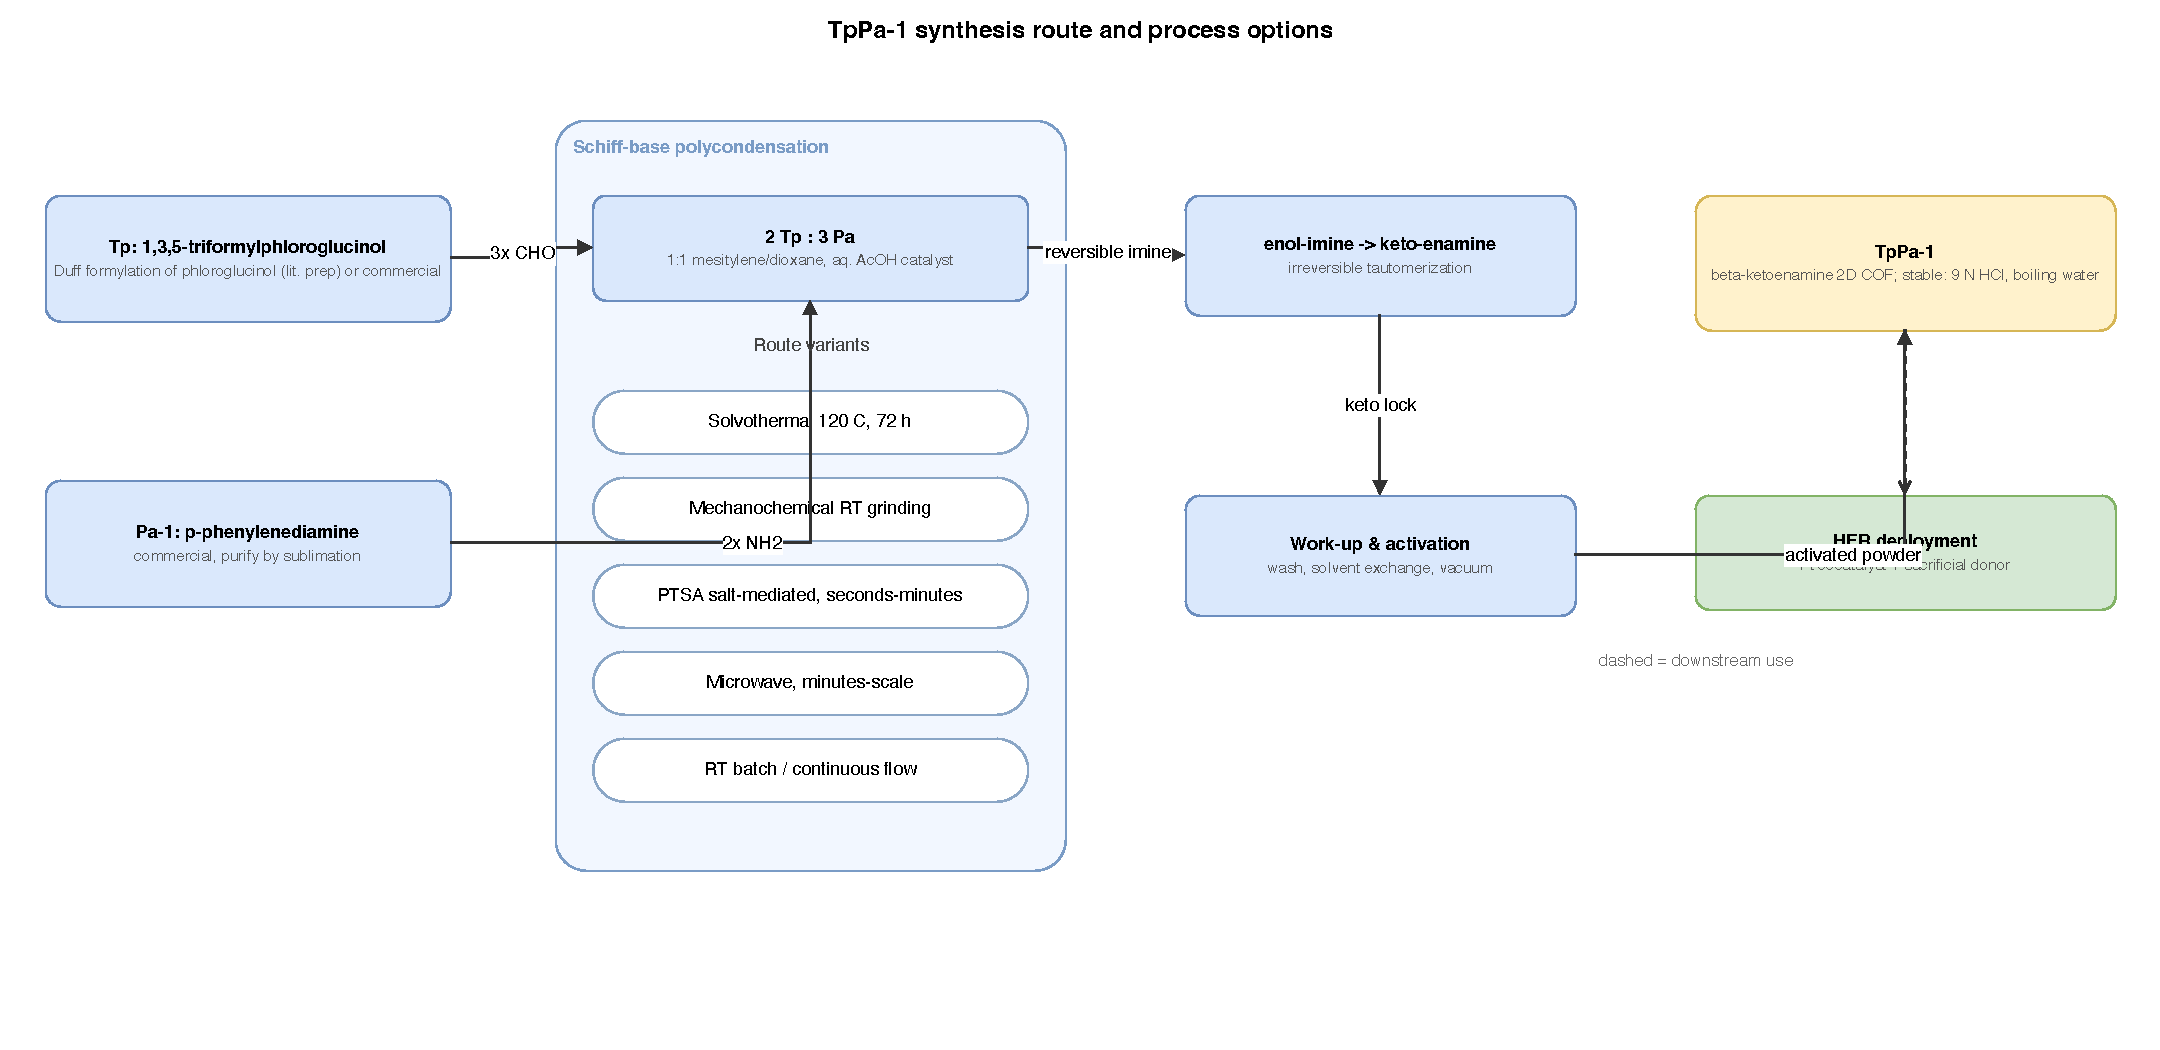
\includegraphics[width=\linewidth]{figures/fig2_tppa1_route.pdf}
  \caption{Synthesis of TpPa-1. Monomers condense via reversible Schiff-base chemistry (route
  variants shown as chips; quantitative comparison in Table~\ref{tab:routes}) and lock into the
  $\beta$-ketoenamine form by irreversible tautomerization, giving an
  acid/base/boiling-water-stable framework deployable for photocatalytic HER.}
  \label{fig:route}
\end{figure}

\textbf{Why TpPa-1, and why these criteria.} The factor chain orders the design requirements:
crystallinity and charge extraction are the prime activity factors~\cite{ghosh2020identification},
and aqueous photocatalysis presupposes hydrolytic stability, which the irreversible
enol$\rightarrow$keto lock provides at the linkage level~\cite{kandambeth2012construction,haase2020solving}.
TpPa-1 is also the only COF in the library with five independently documented synthesis routes
(Table~\ref{tab:routes}), making it the strongest available testbed for evidence-based process
selection~\cite{kandambeth2012construction,biswal2013mechanochemical,karak2017constructing,wei2015the,peng2016room,xu2026structural}.

\textbf{Baseline protocol (decision: solvothermal R1).} Monomer quality first: Pa-1 is
purified (sublimation) immediately before use --- a chemical-practice inference consistent with
the observation that monomer solubility and purity enable mild-condition
growth~\cite{peng2016room}; Tp is purchased or prepared by the literature Duff-type formylation
of phloroglucinol~\cite{kandambeth2012construction}. Condensation follows the origin protocol
(1:1 mesitylene/dioxane, aqueous AcOH, 120~$^\circ$C, 72~h, sealed
tube)~\cite{kandambeth2012construction}, chosen over the four alternatives because it carries
the richest characterization record against which optimized batches can be compared
(Table~\ref{tab:routes}). Work-up uses solvent washing, solvent exchange, and vacuum
activation~\cite{kandambeth2012construction,karak2017constructing}. Deployment for HER follows
the TpPa-COF-X benchmark configuration (in-situ Pt photodeposition, sacrificial
donor)~\cite{sheng2019effect}, with Pt speciation tunable as an independent
factor~\cite{dong2021platinum,li2022in}.

\textbf{Optimization O1 --- microwave heating.} Replacing oven heating with microwave
irradiation reduces reaction time from 72~h to 1~h and temperature from 120 to 100~$^\circ$C
while \emph{increasing} the BET surface area from 152 to 725~m$^2$\,g$^{-1}$ in the direct
comparison~\cite{wei2015the,grenu2020microwave} --- a 98.6\% time reduction and a
$\sim$4.8$\times$ porosity gain. The documented caveat (solvothermal beats microwave for
transimination-based upgrading of $\beta$-ketoenamine COFs~\cite{grenu2020microwave}) is
recorded in the decision table: O1 optimizes the \emph{direct} route, not every quality
pathway.

\textbf{Optimization O2 --- green-solvent continuous flow.} The solvent-thermodynamics
framework (CHEM21 greenness, Hansen parameters, free energy of solvation) selects diacetin;
flow-derived TpPa-1 reaches a BET area of 418~m$^2$\,g$^{-1}$, a 30-fold space-time-yield
increase, and an 89\% reduction in specific energy versus batch in the same
solvent~\cite{xu2026structural}. Feasibility rests on the demonstrated room-temperature growth
of TpPa-1 with solvothermal-grade quality and on the flow precedent of
703~kg\,m$^{-3}$\,day$^{-1}$~\cite{peng2016room}. A salt-mediated seconds-scale route is held
in reserve for crystallinity rescue at scale~\cite{karak2017constructing}, with
amorphous-to-crystalline reconstruction as a further fallback
paradigm~\cite{zhang2022reconstructed}.

\textbf{Thermodynamic feasibility audit.} Literature-supported statements: (i) the route is a
reversible imine equilibrium (error-correcting, crystallinity-enabling) feeding an irreversible
tautomerization whose keto product is the only observed form --- a thermodynamic
sink~\cite{kandambeth2012construction}; (ii) retained crystallinity in 9~N HCl and boiling
water evidences the depth of that sink~\cite{kandambeth2012construction,biswal2013mechanochemical};
(iii) moderate-solvation media thermodynamically balance reversibility against crystallite
growth~\cite{xu2026structural}; (iv) the general reversibility--crystallinity--stability
trade-off frames why this two-stage design is necessary at
all~\cite{haase2020solving,zhang2022reconstructed}. Quantities \emph{not} reported in the
library --- keto/enol tautomer energetics, per-bond condensation free energy, periodic
formation and stacking energies, monomer solvation free energies --- are deliberately left as a
to-be-computed list with recommended DFT setups (dispersion-corrected hybrid functionals with
implicit solvation for molecular models; dispersion-corrected periodic PBE for the framework;
COSMO-RS for solvation screening) rather than asserted numerically. No numeric value in this
section originates outside the cited sources.

\textbf{Validation and characterization plan.} Every batch is judged against
literature-anchored acceptance criteria: powder X-ray diffraction against the simulated
pattern establishes crystallinity~\cite{kandambeth2012construction}; FT-IR and $^{13}$C
CP-MAS NMR must show the keto-form signature that certifies complete
tautomerization~\cite{kandambeth2012construction}; nitrogen sorption benchmarks porosity
against the 725~m$^2$\,g$^{-1}$ (microwave) and 418~m$^2$\,g$^{-1}$ (flow) reference
values~\cite{grenu2020microwave,xu2026structural}; and a 9~N HCl / boiling-water soak with
post-treatment diffraction reproduces the origin stability test~\cite{kandambeth2012construction}.
Stacking disorder during photocatalytic cycling is monitored as a separate failure mode,
following the operando evidence~\cite{zhou2021peg}. Because the three production routes (R1,
O1, O2) will be characterized under one protocol and then deployed under the same HER
configuration~\cite{sheng2019effect}, the plan doubles as the seed experiment for gap G4 ---
the missing route$\rightarrow$crystallinity$\rightarrow$HER chain
(Sec.~\ref{sec:challenges})~\cite{ghosh2020identification}.

\textbf{Safety and integration notes.} The deliverable protocol carries a mandatory hazard
table (diamine sensitizer, dioxane peroxide former, sealed-vessel pressure, microwave-rated
reactors only~\cite{grenu2020microwave}, H$_2$/O$_2$ explosion limits during photocatalysis,
acid handling for in-house Tp preparation). A retrosynthesis-backend integration demo (stub
provider) is included in the project state \emph{explicitly labeled as demonstration data, not
chemical conclusions}; all chemistry above traces to the audited literature.
